\section{Project management}

% Include a timetable (in 2 week chunks) for the remainder of the academic year, up until the submission deadline.

\subsection{The Updated Timeline}
Although the project is on track to meet the schedule set out in the specification, alterations to the schedule have been made. The most major change stems from the realisation that the generation and radio message processing systems can be developed simultaneously, and make sense to be developed in this way. Therefore these two activities have been extended until mid December and been recorded as simultaneous. This has pushed back other tasks, but after researching speech input and taking into account the simple approach decided on, this task has been shortened in duration. Ensuring compliance with the CAP413 manual has also been reduced in duration, given that this will be a brief pass looking over the system's responses and checking them against the manual. Full compliance is was not a stated requirement of the system. The evaluation day has also been marked on the schedule, which will involve getting user feedback from technical users unfamiliar with the project. This feedback can be used to make improvements but these will be made during the execution of the remaining tasks so are not shown on the updated GANTT chart.

\begin{figure}[H]
    \centering
	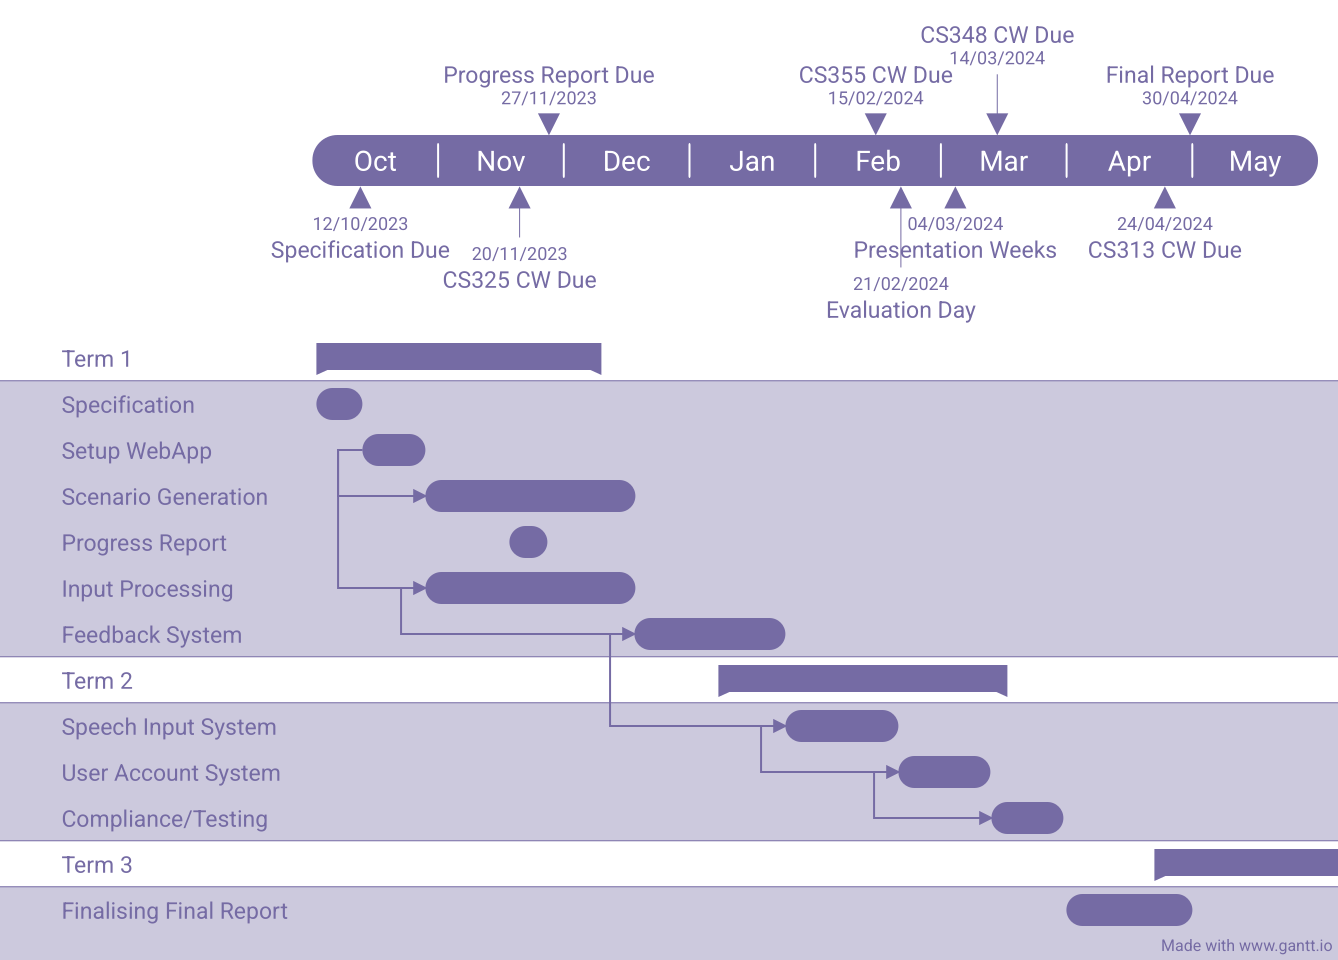
\includegraphics[scale = 0.3]{../document-resources/images/second-gantt}
    \label{progress-report-gantt}
    \caption{Current project timeline.}
\end{figure}

\subsection{Improvements to Working Methods}
No major issues have been encountered so far with the project, but a few changes to working methods will be made to ensure project success. 
\begin{itemize}
    \item More frequent communication with the client will ensure that the features required are correctly implemented once they reach a testable state. The client is the subject expert, and communication will reduce time spent on subject research.
    \item Less time will be spent trying to reinvent the wheel - if a freely available library exists which solves a problem, it should be tried before writing a new solution. Time was previously wasted on specific UI features which ended up being replaced by library code.
    \item Work on deliverable project documents will be started earlier than they have been so far to smooth out the workload. Two large coursework deadlines being close to one another has not been handled as well as it should have been.
\end{itemize} 

\subsection{System Evaluation and Testing}
As mentioned in the project specification, the project's success will be determined by whether all high priority objectives are met. To verify this, various tests will be utilised. These will be written when each system component is near its final iteration, in order to avoid having to rewrite tests every time major changes occur. The following sections provide an overview of the testing that will be required, but a formal plan has not been developed at this stage.

\subsubsection{Testing the Web App}
All UI components, including radio, transponder, and map will be tested via unit tests, as will be the radio call input and output components. Once individual components are passing all tests, they will be tested together to ensure individual settings can be set by the system, and the current setting can be compared against a system state. Automating these tests will be explored if a suitable UI testing library can be found.

\subsubsection{Testing the R/T Web Server}
All radio calls will be tested with both valid and invalid states and calls, and fuzzing will be used to ensure reduce missed system issues. Fuzzing is the process of providing randomised data to an API which are correct enough to not be outright rejected by the input system, an hence expose deeper logic issues. The rust-fuzz library provides a simple interface for performing these tests \cite{rust-fuzz}. The generation will also be tested here by providing various seeds and checking correctness, all of the possible options can be generated, and that the scenarios feel 'random' enough. This last test will be very subjective, as 'random feeling' is very hard to objectively measure. Humans often perceive true randomness in software, for example in the case of the original Spotify shuffle algorithm, as not random \cite{spotify-shuffle}. As the target here is for the system to feel random, as to not annoy users, user feedback may be required.

\subsubsection{Full System Tests}
This will be performed in a similar way to the UI tests, but will test how the whole system responds to correct and incorrect radio calls and radio/transponder settings. 